\documentclass[12pt]{report}
\usepackage{scribe,graphicx,graphics}
\usepackage{subcaption}


\course{MIT 22.213} 	
\coursetitle{Nuclear Reactor Kinetics}	
\semester{Spring 2015}
\lecturenumber{3}	
\lecturedate{}		


% Insert your name here!
\scribe{Geoffrey Gunow}

\begin{document}
	
	
	\maketitle
	
	\paragraph{Intro: Code Design}
	\subparagraph{SWIG Python/C++ Structure}
	In this problem set, I solve the neutron diffusion problem for reactor kinetics in a C++ object-oriented framework. Inputs and outputs are communicated with a SWIG wrapper to Python so that while all the heavy lifting is done in C++, input files are created with simple python scripts. Inside the C++ framework I have created my own sparse matrix solver to handle optimized matrix vector multiplication, matrix addition, and stationary linear solvers (Point Jacobi, Gauss-Seidel, Optimal SOR). The default linear solver is Optimal SOR as it is by far the fastest of the three stationary methods implemented. This code has been written for \textbf{general multi-group}.
	
	\subparagraph{Matrix Formulation}
	In the previous problem set, we looked at steady state problems which had the form of a generalized eigenvalue equation
	\begin{equation}
	A \phi = \frac{1}{k} F \phi
	\end{equation}
	where $A$ is the loss matrix, $F$ is the fission matrix, $k$ is the eigenvalue, and $\phi$ is the flux solution. It is important to note that the loss matrix $A$ has many different contribution terms such as absorption, diffusion, and scattering. In solving reactor kinetics problems it is often advantageous to split these contributions into their own matrices so that changes in each physical parameter can be treated separately. For instance, common transient cases involve an increase or decrease of the absorption cross-section in a region. Therefore we re-write the loss matrix $A$ as
	\begin{equation}
	A = \Sigma_S + \Sigma_A + \hat{D}
	\end{equation}
	where $\Sigma_S$ accounts for all the scattering contributions, $\Sigma_A$ accounts for all the absorption contributions, and $\hat{D}$ accounts for the diffusion terms. With this form, if just one matrix needs to be changed during a time step, only that individual matrix needs to be altered. 
	
	In reactor kinetics we are interested in solving equations of the form
	\begin{equation}
	(\hat{A} - \hat{F}) \phi = S
	\end{equation}
	where $\hat{A}$ is the modified $A$ matrix, $\hat{F}$ is the modified $F$ matrix, $S$ is the lagged neutron time absorption term. Each of matrices will be explained in further detail shortly. To understand where these matrices come from we first need to revert to the time dependent multi-group diffusion equation:
	\begin{eqnarray}
	\frac{\partial}{\partial t} \left\langle \frac{1}{v_g(\vec{r},t)} \phi_g(\vec{r},t) \right\rangle = \nabla D_g(\vec{r},t) \nabla \phi_g(\vec{r},t) - \Sigma_{t,g}(\vec{r},t) \phi_g(\vec{r},t) + \sum_{g'=1}^{G} \Sigma_{s,g'\rightarrow g} (\vec{r},t) \phi_{g'}(\vec{r},t) \nonumber \\ 
	+ \left[ 1- \beta(\vec{r},t) \right] \frac{\chi_g^p}{k_{crit}} \sum_{g'=1}^{G} \nu \Sigma_{f,g'}(\vec{r},t) \phi_{g'}(\vec{r},t) + \sum_{i=1}^{I} \chi_{i,g}^d \lambda_i C_i(\vec{r},t) \nonumber
	\end{eqnarray}
	The variables in the equation take their standard definitions. For more information, see the previous problem set solution and Alan Hebert's textbook. In this equation, neutron precursors $C_i$ are present. They are governed by
	\begin{equation}
	\frac{\partial}{\partial t} C_i(\vec{r},t) = -\lambda_i C_i(\vec{r},t) + \frac{\beta_i(\vec{r},t)}{k_{crit}} \sum_{g'=1}^{G} \nu \Sigma_{f,g'}(\vec{r},t) \phi_{g'}(\vec{r},t).
	\end{equation}
	They can be substituted into the diffusion equation if we use a simple finite difference estimate of time derivatives. As with the previous assignment, the spatial gradients are computed using modified diffusion coefficients $\hat{D_g}$. The resulting equations produce matrices $\hat{A}$ and $\hat{F}$ along with vector $S$.
	
	The modified loss matrix $\hat{A}$ is defined as
	\begin{equation}
	\hat{A} = \Sigma_S + \hat{\Sigma}_A + \hat{D}
	\end{equation}
	where $\Sigma_S$ and $\hat{D}$ take their same definitions as in the steady state equation. The only caveat is that they need to be evaluated at the time step of interest. This may mean an interpolation. Note that $\Sigma_A$ is a diagonal matrix. The modified version for reactor kinetics is again a diagonal matrix but includes the addition of a ``time absorption'' component such that
	\begin{equation}
	\hat{\Sigma}_{A,g}(\vec{r}) = \left\langle \Sigma_{A,g}(\vec{r}) + \frac{1}{v_g(\vec{r}) \Delta_t} \right\rangle
	\end{equation}
	where $\Delta_t$ is the time step. The $F$ matrix is also modified to $\hat{F}$ to account for temporal effects. Whereas the components of $F$ were previously defined to capture neutron production from fission as
	. 
	\begin{equation}
	F_g(\vec{r}) = \chi_g \sum_{g'=1}^{G} \nu \Sigma_{f,g'}(\vec{r}) \phi_{g'}(\vec{r})
	\end{equation}
	These components are transformed so that
	\begin{equation}
	\hat{F}_g(\vec{r}) = \left(\frac{\chi^p_g\left[1- \beta(\vec{r})\right]}{k_{crit}} +  \sum_{i=1}^I \frac{\chi^d_g\beta_i(\vec{r}) \lambda_i \Delta_t}{(1+\lambda_i \Delta_t) k_{crit}} \right) \sum_{g'=1}^{G} \nu \Sigma_{f,g'}(\vec{r}) \phi_{g'}(\vec{r}).
	\end{equation}
	
	Next, we form the right hand side of our problem, the vector $S$. The terms in this vector are formed \textbf{using the flux from the previous time step}. Therefore, this term is lagged, much like the source term in the steady state eigenvalue computations.
	\begin{equation}
	S_g = \left\langle \frac{\phi_g(\vec{r,t_n})}{v_g(\vec{r}) \Delta_t} +  \sum_{i=1}^I \lambda_i \frac{\chi^d_g C_i(\vec{r},t)}{(1+\lambda_i \Delta_t)} \right\rangle
	\end{equation}
	
	Lastly, we need a way to calculate precursor concentrations since they are used in both $\hat{F}$ and $S$. The neutron precursors $C_i(\vec{r},t_{n+1})$ can be calculated as
	\begin{equation}
	C_i(\vec{r},t_{n+1}) = \frac{\beta_i(\vec{r}) \Delta_t}{(1 + \lambda_i \Delta_t) k_{crit}} \sum_{g=1}^{G} \nu \Sigma_{f,g} \phi_g (\vec{r},t_{n+1})  + \frac{C_i(\vec{r}, t_n)}{1+\lambda_i \Delta_t}.
	\end{equation}
	
	With this formulation we can solve for the simple linear solution of
	\begin{equation}
	T \phi = S
	\end{equation}
	at every time step using a linear solver such as SOR where
	\begin{equation}
	T = \hat{A} - \hat{F}.
	\end{equation}
	
	\paragraph{Part A: Delayed Critical Bank Withdrawal}
	In this problem, the reactor kinetics solver is used to solve for a case in which a transient occurs without becoming prompt super-critical.  A control rod is withdrawn and then inserted back to stop the transient. Since there is no thermal hydraulic feedback, the re-insertion of the rod is required to stop the transient. To determine the control rod worth, we can calculate the static rod worth using steady state eigenvalue solutions to the inserted and withdrawn rod geometries. The static reactivity $\rho_\text{static}$ can be computed as 
	\begin{equation}
	\rho_\text{static} = \frac{\Delta k}{k}
	\end{equation}
	where $k$ is the calculated eigenvalue of the initial state and $\Delta k$ is the difference in the eigenvalues between the initial and final states. The resulting reactivity is calculated to be $\boxed{\rho_\text{static} = 0.3732 \beta}$.
	
	\begin{figure}[ht]
		\centering
		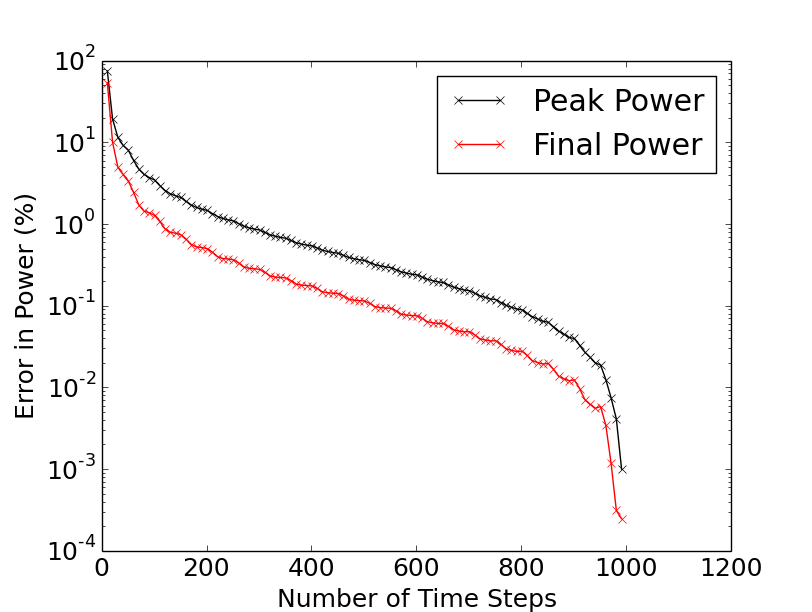
\includegraphics[width=.9\linewidth]{figs/partA_convergence.png}
		\caption{Relative error in power as the number of time steps is varied for part A. The reference is a solution with 1000 time steps. All simulations use a 1.0 cm spatial mesh.}
		\label{fig::partAconv}
	\end{figure}
	
	Next, the time step needs to be refined to converge the problem. In order to determine the appropriate time step, increasingly smaller values are chosen until the difference in solution peak power and final power is sufficiently low. The results are plotted in Fig.~\ref{fig::partAconv}. This plot shows very smooth convergence. In order to achieve this the user mush be careful to include the $t=10.0$ as a solution point under the input mesh spacing. If $t=10.0$ is not included, the true peak will not be captured and there will be a large oscillation overlaid on the convergence. Also notice that the final power converges faster than the peak power. This seems to be intuitive since the final power can seem difficult to capture. Using this result we see that convergence of the peak power to within 1\% requires 270 time steps, associated with a time step size $\Delta_t = 0.185$ whereas convergence of the final power to within 1\% requires 120 time steps, associated with a time step size of $\Delta_t = 0.417$. These results are displayed in Table~\ref{tab::timestepA}.
	
		\begin{table}[ht]
			\begin{center}
				\caption{\label{tab::timestepA} Required number of time steps and time step size to converge part A}
				\begin{tabular}{lll}
					\hline
					Quantity & Number of Steps & Time Step Size (s) \\
					\hline
					Peak Power & 270 & 0.185\\
					Final Power & 120 & 0.417\\
					\hline
				\end{tabular}
			\end{center}
		\end{table}
	
	\clearpage
	The solution to part A for the converged time steps is shown in Fig.~\ref{fig::partA_power}.
	\begin{figure}[ht]
		\centering
		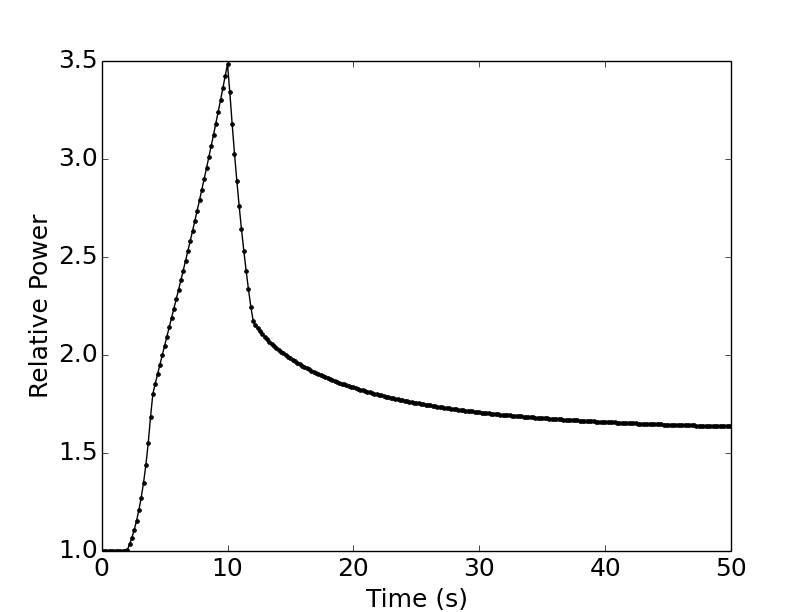
\includegraphics[width=.9\linewidth]{figs/partA_trans271.png}
		\caption{Relative reactor power over time after the withdrawal and re-insertion of a central control rod. The solution uses 270 time steps of 0.185 seconds with a 1.0 cm mesh.}
		\label{fig::partA_power}
	\end{figure}
	
	Next we revisit the time step refinement by multiplying the time step length by 1, 2, 4, 8, 16, 32, and 64 to observe the deterioration of the solution. The result is shown in Fig.~\ref{fig::partA_timestep}.
	\begin{figure}[ht]
		\centering
		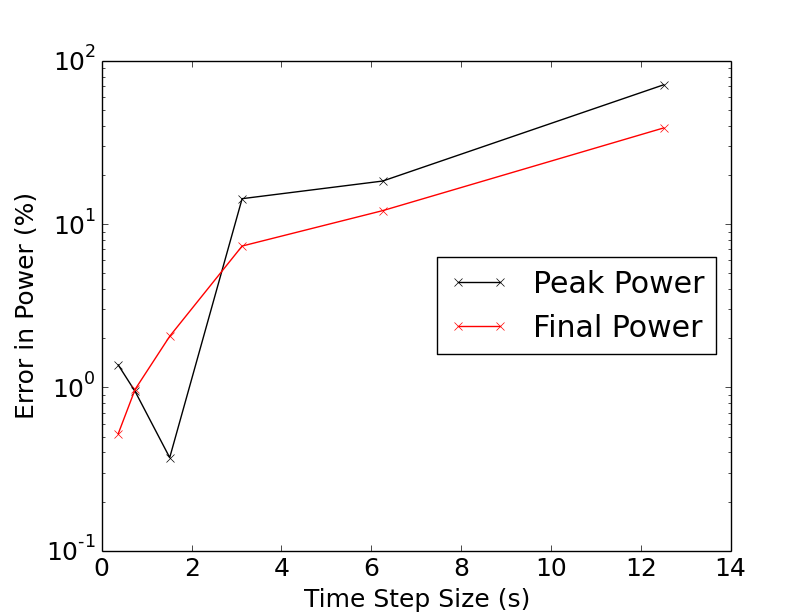
\includegraphics[width=.7\linewidth]{figs/partA_timeStep.png}
		\caption{Effect of time step size on solution error for part A. The reference solution uses 270 time steps of 0.185 seconds with a 1.0 cm mesh.}
		\label{fig::partA_timestep}
	\end{figure}
	
		Lastly, we quantify the error incurred from using a coarser mesh. Whereas our reference solution used a 1.0 cm mesh, we compare with mesh spacings of 2.0 cm, 5.0 cm, and 10.0 cm. This is shown in Fig.~\ref{fig::partA_spatial}.
			\begin{figure}[ht]
				\centering
				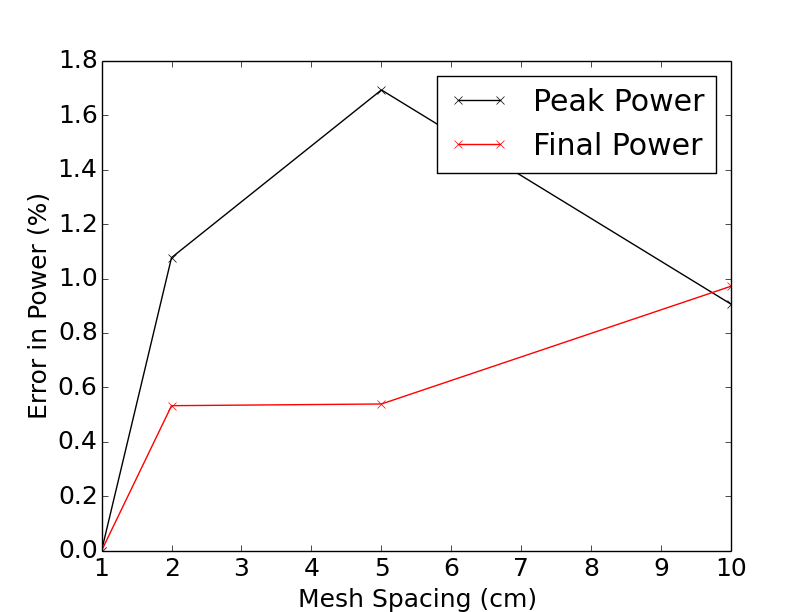
\includegraphics[width=.7\linewidth]{figs/partA_spatial.png}
				\caption{Effect of mesh spacing on solution error for part A. The reference solution uses 270 time steps of 0.185 seconds with a 1.0 cm mesh.}
				\label{fig::partA_spatial}
			\end{figure}
	

\clearpage
\paragraph{Part B: Super-prompt Critical} Now we repeat our previous investigation on a problem that becomes super-prompt critical, meaning that delayed neutrons have almost no effect on the solution. This causes fast exponential growth of the power. Once again, we calculate rod worth and find the static reactivity $\boxed{\rho_\text{static} = 1.241 \beta}$.

The same process as before is used to choose a appropriate time step. The convergence of peak power and final power is shown in Fig.~\ref{fig::partB_convergence}. 

	\begin{figure}[ht]
		\centering
		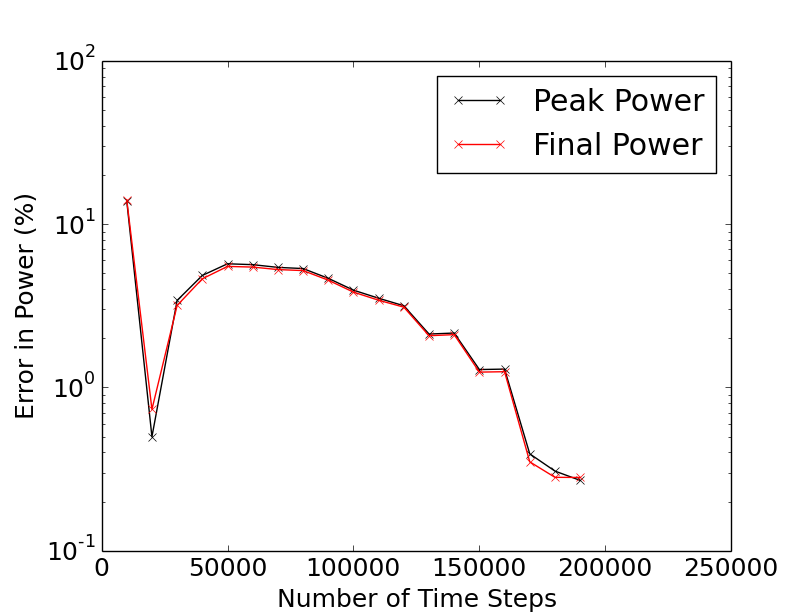
\includegraphics[width=.9\linewidth]{figs/partB_convergence.png}
		\caption{Relative error in power as the number of time steps is varied for part B. The reference is a solution with $2\times10^6$ time steps. All simulations use a 1.0 cm spatial mesh.}
		\label{fig::partB_convergence}
	\end{figure}

Note that the convergence is far less smooth than before. Also, many more time steps are needed to converge this problem. For determining the appropriate time step, notice that there is a sharp drop in error at $2 \times 10^4$ time steps, associated with a time step of 0.1 ms. At this point, both the peak power and final power show less than 1\% error. However, this sharp drop seems to be an artifact of the convergence and should not be trusted. Therefore, a time step of $1.176 \times 10^{-5}$ associated with $1.7 \times 10^5$ time steps is chosen. This point also shows less than 1\% error on both the peak power and the final power.  It might seem odd that the final power converges at the same rate as the peak power. However, it is important to remember that the peak power has a strong impact on the final power through the formation of precursors so an error in the peak power should directly impact the estimate of the final power. The number of time steps and time step size required to produce errors within 1\% for both the peak power and final power and shown in Table~\ref{tab::timestepB}
	
	\begin{table}[ht]
		\begin{center}
			\caption{\label{tab::timestepB} Required number of time steps and time step size to converge part B}
			\begin{tabular}{lll}
				\hline
				Quantity & Number of Steps & Time Step Size (s) \\
				\hline
				Peak Power & $1.7\times10^5$ &  $1.176 \times 10^{-5}$\\
				Final Power & $1.7\times10^5$ &  $1.176 \times 10^{-5}$\\
				\hline
			\end{tabular}
		\end{center}
	\end{table}


The power profile produced from the converged solution is shown in Fig.~\ref{fig::partB_power}.
	\begin{figure}[ht]
		\centering
		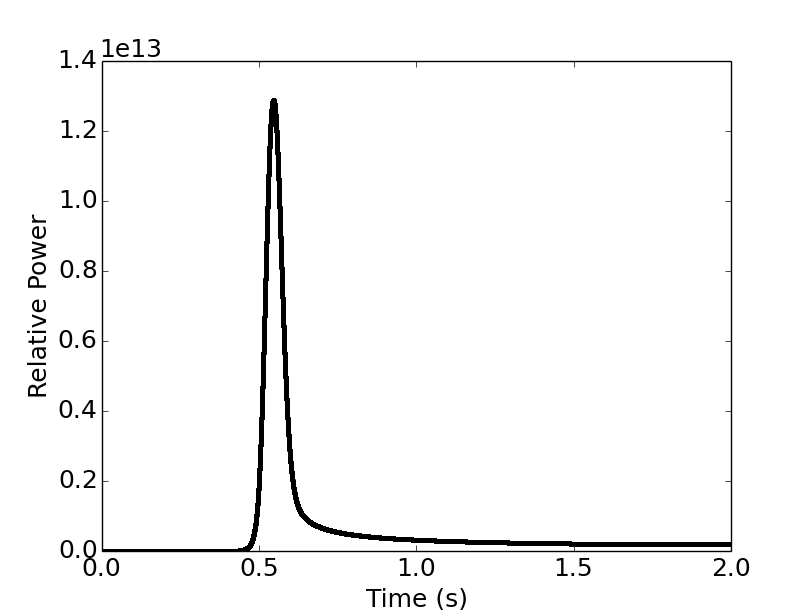
\includegraphics[width=.9\linewidth]{figs/partB_trans17.png}
		\caption{Relative reactor power over time after a prompt super-critical transient and a central control rod scram. The solution uses $1.7\times10^5$ time steps of  $1.176 \times 10^{-5}$ seconds with a 1.0 cm mesh.}
		\label{fig::partB_power}
	\end{figure}

Lastly, the time step and spatial convergence are presented in Fig.~\ref{fig::partB_timestep} and Fig.~\ref{fig::partB_spatial} respectively.


	\begin{figure}[ht]
		\centering
		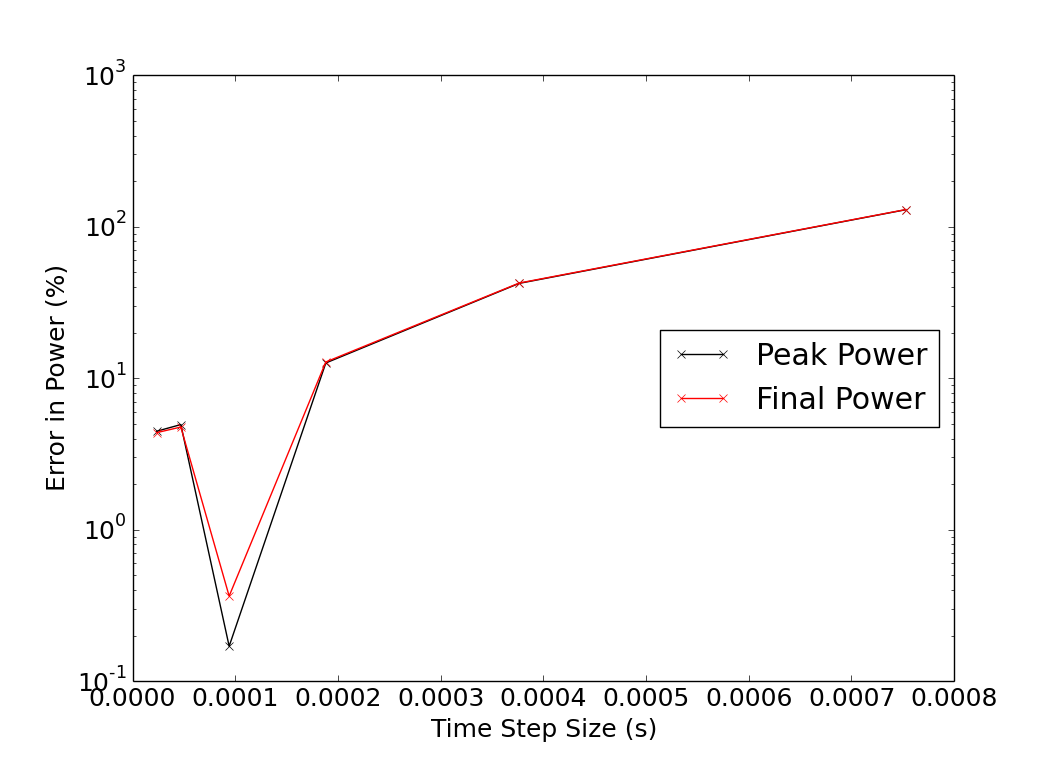
\includegraphics[width=.7\linewidth]{figs/partB_timeStep.png}
		\caption{Effect of time step size on solution error for part B. The reference solution uses $1.7\times10^5$ time steps of  $1.176 \times 10^{-5}$ seconds with a 1.0 cm mesh.}
		\label{fig::partB_timestep}
	\end{figure}

	\begin{figure}[ht]
		\centering
		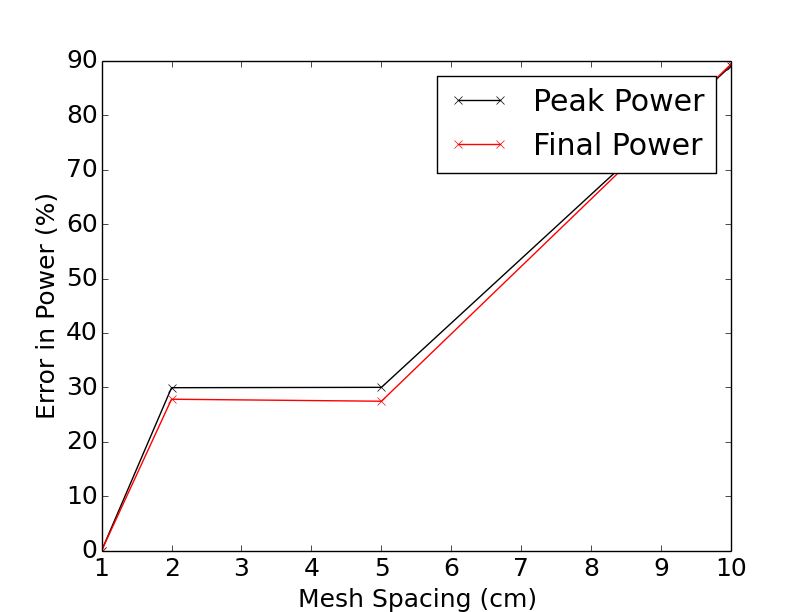
\includegraphics[width=.7\linewidth]{figs/partB_spatial.png}
		\caption{Effect of mesh spacing on solution error for part B. The reference solution uses $1.7\times10^5$ time steps of $1.176 \times 10^{-5}$ seconds with a 1.0 cm mesh.}
		\label{fig::partB_spatial}
	\end{figure}
\end{document}